\documentclass{article}

\usepackage{amsmath,amssymb,amsthm,graphicx,subfigure}

\pagestyle{myheadings}

\pdfpagewidth 8.5in
\pdfpageheight 11 in

\setlength\topmargin{0in}
\setlength\textheight{8.5in}
\setlength\textwidth{6.5in}
\setlength\oddsidemargin{0in}
\setlength\evensidemargin{0in}

\newcommand{\suchthat}{\ni}
\newcommand{\onlyif}{\Longleftrighttriangle}
\newcommand{\definedby}{\triangleq}
\newcommand{\union}{\bigcup}
\newcommand{\intersect}{\bigcap}
\newcommand{\where}{\mid}
\newcommand{\inverse}{\overline}

\title{CIT 596 Homework 3}
\author{Steven Tomcavage\\stomcava@seas.upenn.edu}
\date{February 17, 2011}

\markboth{\hfill Steven Tomcavage }{\hfill Steven Tomcavage }

\begin{document}

\maketitle

\section{Exercise 1.13}

Give a DFA that recognizes the language $F$ where $F$ is the language of all
strings over $\{0, 1\}$ that do not contain a pair of $1$s which are separated
by an odd number of symbols.

\begin{figure}[h!]
	\centering
	\subfigure[The NFA $A$ accepts $\inverse{F}$] {
		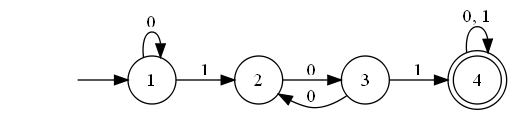
\includegraphics[height=1.0in]{1_13_a.png}
	}
	\subfigure[The DFA $B$ accepts $F$] 
	{
		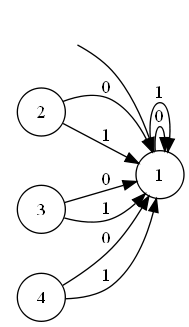
\includegraphics[height=1.0in]{1_13_b.png}
	}
	\caption{DFA for Exercise 1.13}
\end{figure}

\section{Exercise 1.16b}

Convert the given NFA (omitted) to a DFA. 

\begin{figure}[h!]
	\centering
	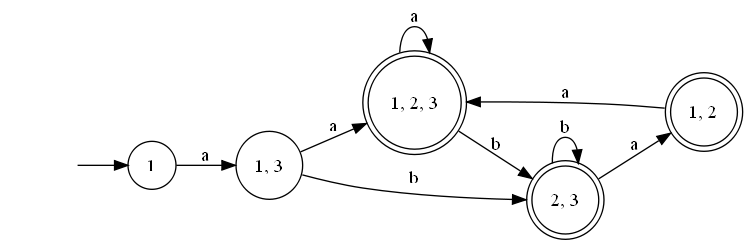
\includegraphics[height=2.0in]{1_16.png}
	\caption{DFA for Exercise 1.16b}
\end{figure}

\section{Exercise 1.17a}

Give an NFA recognizing the language $(01 \union 001 \union 010)^\star$.

\begin{figure}[h!]
	\centering
	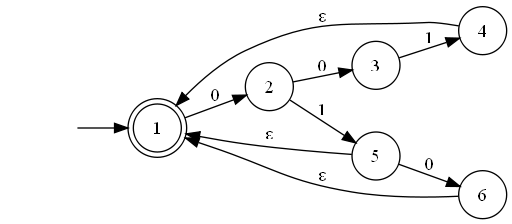
\includegraphics[height=2.0in]{1_17_a.png}
	\caption{DFA for Exercise 1.17a}
\end{figure}

\section{Exercise 1.17b}

Convert the NFA from Exercise 1.17a to an equivalent DFA.

TODO

\section{Exercise 1.19b}

Convert the following regular expression to an NFA: $(((00)^\star (11)) \union
01)^\star$.

\begin{figure}[h!]
	\centering
	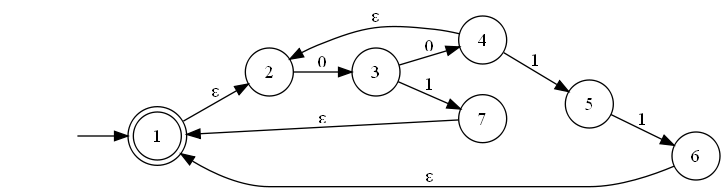
\includegraphics[height=1.5in]{1_19.png}
	\caption{DFA for Exercise 1.19b}
\end{figure}

\section{Exercise 1.21b}

Convert the following NFA to a regular expression.

TODO

\section{Exercise 1.28c}

Convert the regular expression $(a \union b^+) a^+ b^+$ to an NFA, given that
$\Sigma = \{a, b\}$.

\begin{figure}[h!]
	\centering
	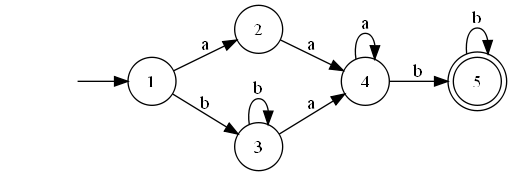
\includegraphics[height=1.5in]{1_28.png}
	\caption{DFA for Exercise 1.28c}
\end{figure}

\section{Exercies 1.29b}

Use the pumping lemma to show that the language $A_2 = \{ \omega \omega \omega
\where \omega \in \{a, b\}^\star \}$ is not regular.

TODO


\end{document}

